\section{Introduction to Security and Cryptology}

\subsection{Ziele der Kryptographie}

\begin{definition}{Ziele der Kryptographie}
    Die Kryptographie verfolgt vier Hauptziele:
    \begin{itemize}
        \item \textbf{Confidentiality} Only readable by desired receiver.
        \item \textbf{Integrity} The receiver can determine if the message has been altered.
        \item \textbf{Authenticity} The receiver can validate its origin.
        \item \textbf{Freshness} The message is new and cannot be resent.
    \end{itemize}
\end{definition}


\subsubsection{Model der Kommunikation und Verschlüsselung}

\begin{definition}{Kommunikationsmodel}

    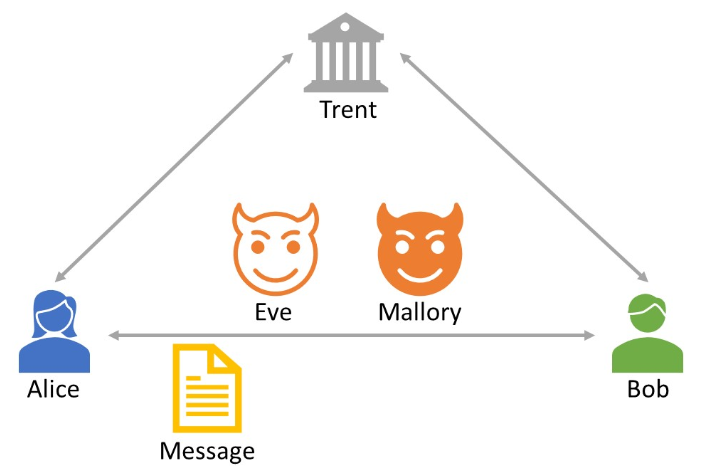
\includegraphics[width=0.7\linewidth]{kommunikationsmodel.png}

    \begin{itemize}
        \item \textcolor{darkblue}{\textbf{Alice}} sendet eine Nachricht an Bob. Dabei sollen die oben genannten Ziele, confidentiality, integrity, authenticity, non-repudiation und freshness erfüllt werden.
        \item \textcolor{darkgreen}{\textbf{Bob}} empfängt die Nachrichten von Allice. Er will überprüfen können, dass die Ziele eingehalten wurden.
        \item \textcolor{darktangerine}{\textbf{Eve}}  ist ein Attacker. Sie kann Nachrichten mitlesen, aber sie nicht verändern.
        \item \textcolor{darkred}{\textbf{Mallory}} ist ein anderer Attacker. Er kann Daten sowohl mitlesen als auch verändern. Er kann auch Nachrichten abfangen und später weitersenden, oder ganz verwerfen. Er kann auch neue Nachrichten generieren.
        \item \textcolor{darkgrey}{\textbf{Trent}} ist eine Drittperson/Instanz, welcher sowohl Alice und Bob vertrauen. Trent unterstützt Alice und Bob bei der sicheren Kommunikation.
    \end{itemize}
\end{definition}

\begin{concept}{Model der Verschlüsselung}
    Um eine vertrauliche Kommunikation zu erreichen, werden Nachrichten vor dem Senden verschlüsselt und nach dem Empfangen wieder entschlüsselt.

    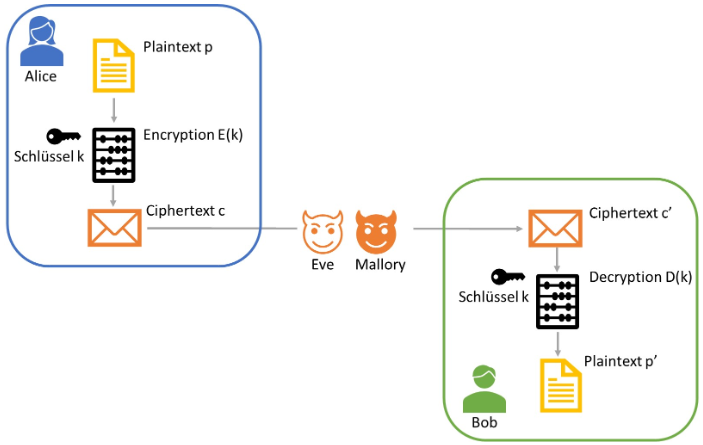
\includegraphics[width=\linewidth]{model_der_verschluesselung.png}

    \begin{itemize}
        \item \textcolor{darkcorn}{\textbf{Plaintext (Klartext):}} Der Plaintext ist der Text, so wie er geschrieben, respektive gelesen werden kann. Er wird mit dem Buchstaben "p" abgekürzt.
        \item \textcolor{darkorange}{\textbf{Ciphertext (Verschlüsselter Text):}} Der Ciphertext ist der Text, welcher durch die Verschlüsselung entsteht. Er wird mit dem Buchstaben "c" abgekürzt.
        \item \textcolor{darkturquoise}{\textbf{Encryption (Verschlüsselung):}} Die Verschlüsselung macht aus dem Plaintext den dazugehörenden Ciphertext. Dazu wird ein Schlüssel verwendet. Die Verschlüsselung kann wie folgt angegeben werden: $c=E[k](p)$. Der Verschlüsselungsalgorithmus selbst ist öffentlich bekannt und kann von allen analysiert werden, um mögliche Schwachstellen zu finden.
        \item \textcolor{darkturquoise}{\textbf{Decryption (Entschlüsselung):}} Die Entschlüsselung macht aus einem Ciphertext den dazugehörenden Plaintext. Dazu wird ein Schlüssel verwendet. Die Entschlüsselung kann wie folgt angegeben werden p' = D[k](c'). Der Entschlüsselungsmechanismus ist öffentlich bekannt und kann von allen analysiert werden, um mögliche Schwachstellen zu finden.
        \item \textcolor{darkpink}{\textbf{Key (Schlüssel):}} Nur mit dem richtigen Schlüssel, kann eine Nachricht richtig entschlüsselt werden. Je nach Art der Verschlüsselung wird derselbe Key für die Verschlüsselung und die Entschlüsselung verwendet (Secret Key Kryptographie) oder es werden unterschiedliche Schlüssel verwendet (Public Key Kryptographie). Damit die Verschlüsselung sicher ist, muss der Schlüssel, welcher für die Entschlüsselung gebraucht wird, geheim bleiben.
    \end{itemize}

    \textbf{Confidentiality} ist erreicht, wenn Eve (und Mallory) den Ciphertext c nicht lesen können. \textbf{Integrity} ist erreicht wenn der von Bob empfangene Plaintext p' dem von Alice gesendeten Plaintext p entspricht, also \textcolor{darkcorn}{\textbf{p' = p}} ist. Authenticity ist erreicht, wenn Bob sicher sein kann, dass die Nachricht von Alice stammt. Non-repudiation ist erreicht, wenn Alice nicht abstreiten kann, dass sie die Nachricht gesendet hat. Freshness ist erreicht, wenn Bob sicher sein kann, dass die Nachricht aktuell ist.
    
\end{concept}

\subsection{Encryption and Properties}

\begin{concept}{Encryption}
    Encryption is a transformation from P (plaintexts) to C (ciphertexts) under control of some key, chosen from K (key space).
    
    The idea is to have a whole family of transformations, where each key gives a different transformation.
    \begin{itemize}
        \item $c = E(k, p) = E_k(p)$
        \item $p = D(k, c) = D_k(c)$
    \end{itemize}
    
    Each transformation must be reversible. It follows that $|C|$ can not be smaller than $|P|$. In fact most often we have $P = C$.
\end{concept}

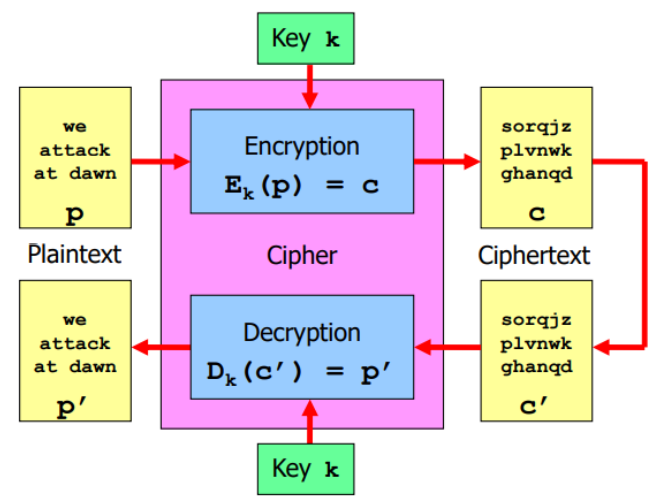
\includegraphics[width=0.6\linewidth]{encryption_decryption.png}

\subsubsection{Attacktypen auf Kryptosysteme}

\begin{remark}
    Die Unterschiede zwischen den Attacken bestehen daraus, auf was der Attacker Zugriff hat.
\end{remark}

\begin{definition}{Ciphertext-only attack}
    Der Attacker kann vom Ciphertext alleine Rückschlüsse auf den Plaintext oder den 
    verwendeten Schlüssel ziehen.
\end{definition}

\begin{definition}{Chosen-ciphertext attack}
    Der Attacker kann Ciphertexte generieren und diese vom System entschlüsseln lassen. 
    Der Attacker bekommt entweder den zum gewählten Ciphertext gehörenden Plaintext 
    (und kann daraus potenziell Rückschlüsse auf den verwendeten Schlüssel machen) 
    oder er bekommt nur Teilinformationen, wie zum Beispiel 
    "Die Entschlüsselung konnte / konnte nicht durchgeführt werden".
\end{definition}

\begin{definition}{Known-plaintext attack}
    Der Attacker kennt sowohl Teile des Plaintext als auch den dazugehörenden Ciphertext (oder zumindest Teile davon). 
    Er kann daraus Rückschlüsse auf andere Plaintexte oder gar den Schlüssel machen.
\end{definition}

\begin{definition}{Chosen-plaintext attack}
    Der Attacker kann Plaintexte wählen, welche er vom System verschlüsseln lassen will. 
    Er erhält dann den dazugehörenden Ciphertext und kann daraus Rückschlüsse auf 
    andere Plaintexte oder gar den Schlüssel machen.
\end{definition}

\begin{definition}{Brute-force attack}
    Der Attacker probiert alle möglichen Schlüssel aus, bis er den richtigen gefunden hat. 
    Dass er den richtigen gefunden hat, erkennt er daran, dass der erhaltene Plaintext sinnvoll erscheint.
\end{definition}

\begin{remark}
    Grundsätzlich können alle Verschlüsselungsalgorithmen mittels brute-force Attacken geknackt werden. 
    Ein wichtiges Evaluationskriterium eines Verschlüsselungsalgorithmus ist also, wie lange eine solche brute-force Attacke im Durchschnitt benötigt. Dieser Anzahl sagt man auch kryptographischer Work Factor.
\end{remark}

\raggedcolumns
\columnbreak

\subsection{Cryptographic Work Factor}

\begin{definition}{Work Factor}
    The number of times it takes to come upon the correct key is called (cryptographic) work factor.
    \begin{itemize}
        \item Work factor (WF) = average number of keys to try
        \item Work factor is usually given in bits: $\log_2(n)$, $n = key\ space\ size$
    \end{itemize}
\end{definition}

\begin{formula}{Entropy}
    Entropy is maximal if all outcomes are equally likely
    $$H = \sum_{i=1}^{n} p(i) \cdot \log_2 \left(\frac{1}{p(i)}\right)$$
    
    $$H_{binary} = \sum_{i=1}^{n} \frac{1}{n} \log_2(n) = \log_2(n)$$
\end{formula}

\begin{concept}{Entropy of Cryptographic Keys}\\
    Cryptographic keys are typically created with random generators, so they can be considered as elements of a random variable.
    
    What's the entropy of a key with 128-bit?
    \begin{itemize}
        \item Independent with equal probability: $128 \cdot 1 = 128$ bits
        \item Dependent with inequal probability: $p(0) = 0.25, p(1) = 0.75 \rightarrow 128 \cdot 0.81 \approx 104$ bits
    \end{itemize}
\end{concept}

\begin{theorem}{Relation between entropy and work factor}\\
    Work Factor $\approx$ entropy, key size = max. entropy $\approx$ max. work factor
\end{theorem}

\subsection{Security Models}

\begin{definition}{Information-theoretically secure}
    Intercepting a ciphertext tells you nothing about the plain
\end{definition}

\begin{definition}{Computationally secure}
    Work factor $\approx$ key entropy
\end{definition}





